  \documentclass{mynotes}

%\geometry{showframe}% for debugging purposes -- displays the margins

\newcommand{\E}{\mbox{E}}
\newcommand{\MSE}{\mbox{MSE}}
\newcommand{\var}{\mbox{var}}


\usepackage{amsmath}
%\usepackage[garamond]{mathdesign}
\usepackage{url}

% Set up the images/graphics package
\usepackage{graphicx}
\setkeys{Gin}{width=\linewidth,totalheight=\textheight,keepaspectratio}
\graphicspath{{graphics/}}

\title[Exercises 6 $\cdot$ SSC 383D]{Exercises 7: Latent-feature models}
%\author[ ]{ }
\date{}  % if the \date{} command is left out, the current date will be used

% The following package makes prettier tables.  We're all about the bling!
\usepackage{booktabs}

% The units package provides nice, non-stacked fractions and better spacing
% for units.
\usepackage{units}

% The fancyvrb package lets us customize the formatting of verbatim
% environments.  We use a slightly smaller font.
\usepackage{fancyvrb}
\fvset{fontsize=\normalsize}

% Small sections of multiple columns
\usepackage{multicol}

% Provides paragraphs of dummy text
\usepackage{lipsum}

% These commands are used to pretty-print LaTeX commands
\newcommand{\doccmd}[1]{\texttt{\textbackslash#1}}% command name -- adds backslash automatically
\newcommand{\docopt}[1]{\ensuremath{\langle}\textrm{\textit{#1}}\ensuremath{\rangle}}% optional command argument
\newcommand{\docarg}[1]{\textrm{\textit{#1}}}% (required) command argument
\newenvironment{docspec}{\begin{quote}\noindent}{\end{quote}}% command specification environment
\newcommand{\docenv}[1]{\textsf{#1}}% environment name
\newcommand{\docpkg}[1]{\texttt{#1}}% package name
\newcommand{\doccls}[1]{\texttt{#1}}% document class name
\newcommand{\docclsopt}[1]{\texttt{#1}}% document class option name

\newcommand{\N}{\mbox{N}}
\newcommand{\thetahat}{\hat{\theta}}
\newcommand{\sigmahat}{\hat{\sigma}}
\newcommand{\betahat}{\hat{\beta}}


\begin{document}

\maketitle% this prints the handout title, author, and date


\section{Projecting downward}

A question one often encounters in statistics is: given a $p$-dimensional vector, how do we project it down into a smaller $k$-dimensional space in a way that preserves as much of the information in the original data as possible? The point is to represent a large amount of information in a tractable, more parsimonious way---in other words, to cut through the clutter.

You already know one way of doing this, namely linear regression.  Given an $n$-dimensional outcome vector $y$ and a matrix of covariates $X$, the fitted values $\hat{y} = X (X^T X)^{-1} X^T y$ (or their equivalents arising from a Bayesian model) involve a projection from $\mathcal{R}^n$ to $\mathcal{R}^p$.  But what if you don't have regressors $X$, only the outcomes $y$?

\subsection{A simple example: projection to $\mathcal{R}$}

Say we have $n$ observations of a $p$-dimensional outcome vector $y_i$. By $Y$, I mean the matrix whose $i$th row is the $i$th observation $y_i^T = (y_{i1}, \ldots, y_{ip})^T$.  (Remember by convention that vectors are column vectors.) Suppose for the moment that every column of $Y$ is standardized to have mean zero and unit variance.

Imagine projecting every observation $y_i$ into a one-dimensional subspace---that is, defining a new scalar outcome $z_i = y_i^T w_1$ for some vector $w_1$.  Presumably $w_1$ should be maximally information-preserving.  The question is how to operationalize this rather loose idea.

\begin{marginfigure}
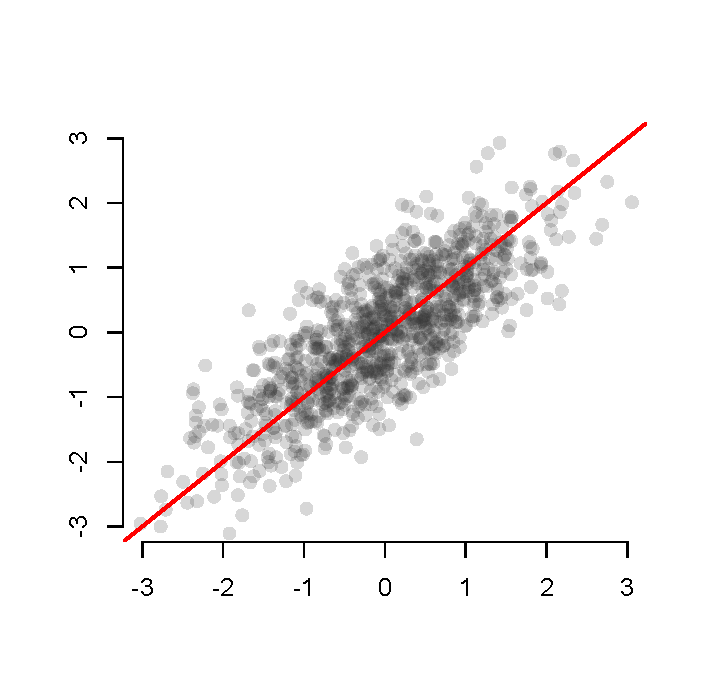
\includegraphics{cloud1.pdf}
\end{marginfigure}

Here's one way: choose $w_1$ so as to \textit{maximize the variance} of the projected values $z_i$.  The intuition for this is straightforward.  In the picture at right, the points can be described fairly well by projecting each one onto the diagonal line and reporting the single number $z_i$.  (Or equivalently, its actual position in $p$-dimensional space, which is $z_i w_1$---though this requires $p$ numbers.)  It's also easy to see that the projected points will have greater variance in this subspace than they would in any other choice of subspace.  Try drawing some other line through the point cloud; you'll see that the projections of the points onto this line would be more scrunched up than along the line I've drawn.

Mathematically, this means choosing $w_1$ such that the projected variance
$$
V_w = \frac{1}{n} \sum_{i=1}^n (z_i - \bar{z})^2 =  \frac{1}{n} \sum_{i=1}^n (y_i^T w_1 - \bar{z})^2
$$
is as large as possible.  Of course, we can blow up the variance to be as large as we want by choosing $w_1$ itself to be huge, so we must constrain it somehow.  A natural constraint is that $w_1$ is a unit vector: $w_1^T w_1 = 1$.

\begin{enumerate}

\item Characterize the relationship between the singular value decomposition of $Y$ and the eigenvalue decomposition of $\frac{1}{n} Y^T Y$.

\item Prove\footnote{Remember that the method of Lagrange multipliers is useful for optimizing under constraints.} that the unit-length $w_1$ which maximizes the projection variance is a left-singular vector of the data matrix $Y$ corresponding to the largest singular value $d_1$.  What is the relationship between $V_w$ and $d_1$?

\item Load the data in ``congress109.csv.''  The rows are members of the 109th U.S.~Congress; the columns are phrases uttered during floor speeches.  Entry $(i,j)$ in the matrix is the number of times member $i$ uttered phrase $j$.  Find the variance-maximizing one-dimensional projection, and compute the location of each member in this one-dimensional space.  (Meet R's built-in routines \verb|svd| and \verb|eigen|.) You've now moved from 1000 pieces of information about each member, to 1.  Consult the information in ``congress109members.csv.''  (You might find R's \verb|merge| command helpful.)  Does location in the  subspace you've defined seem to correlate with relevant political facts about each member?

\item Since each projected value is $z_i = y_i^T w_1$, we can write the whole column vector of $z_i$'s as $Z = Y w_1$, and the residuals from this projection as $R = Y - Z w_1^T$.  Each row of $R$ is the residual vector for the $i$th case, after the projection.

Now imagine applying the same procedure as above to the residuals: that is, finding the maximum-variance projection of each residual vector, defined by some new vector $w_2$.  Prove that $w_2$ is the singular vector of the original data matrix $Y$ corresponding to the second largest singular value $d_2$.

\end{enumerate}

\end{document}

